\chapter{Comparison to Other Data}
\label{cha:Comparison}

A similar measurement has been published by the CLAS Collaboration using \mbox{E1-6} data~\cite{Osipenko09}.
However, it only measures the $\pi^+$ channel and has a more limited kinematic range.
A comparison for the $\pi^+$ channel in overlapping kinematic ranges is done here.
In order to have a meaningful comparison, the binning scheme used here was temporarily changed to match that of~\cite{Osipenko09}.
Figure~\ref{fig:osipenkoComparisonVPT2_2zBins} shows the comparison between E1-f (red points) and E1-6 (black points) as a function of $P_{h\perp}^2$ for two $z$ bins ($0.29 < z < 0.32$ (left column) and $0.32 < z < 0.35$ (right column)) for the $\pi^+$ channel.
The results show clear agreement, both qualitatively and quantitatively, implying good consistency between measurements.
%
\begin{sidewaysfigure}[htp]
\centering
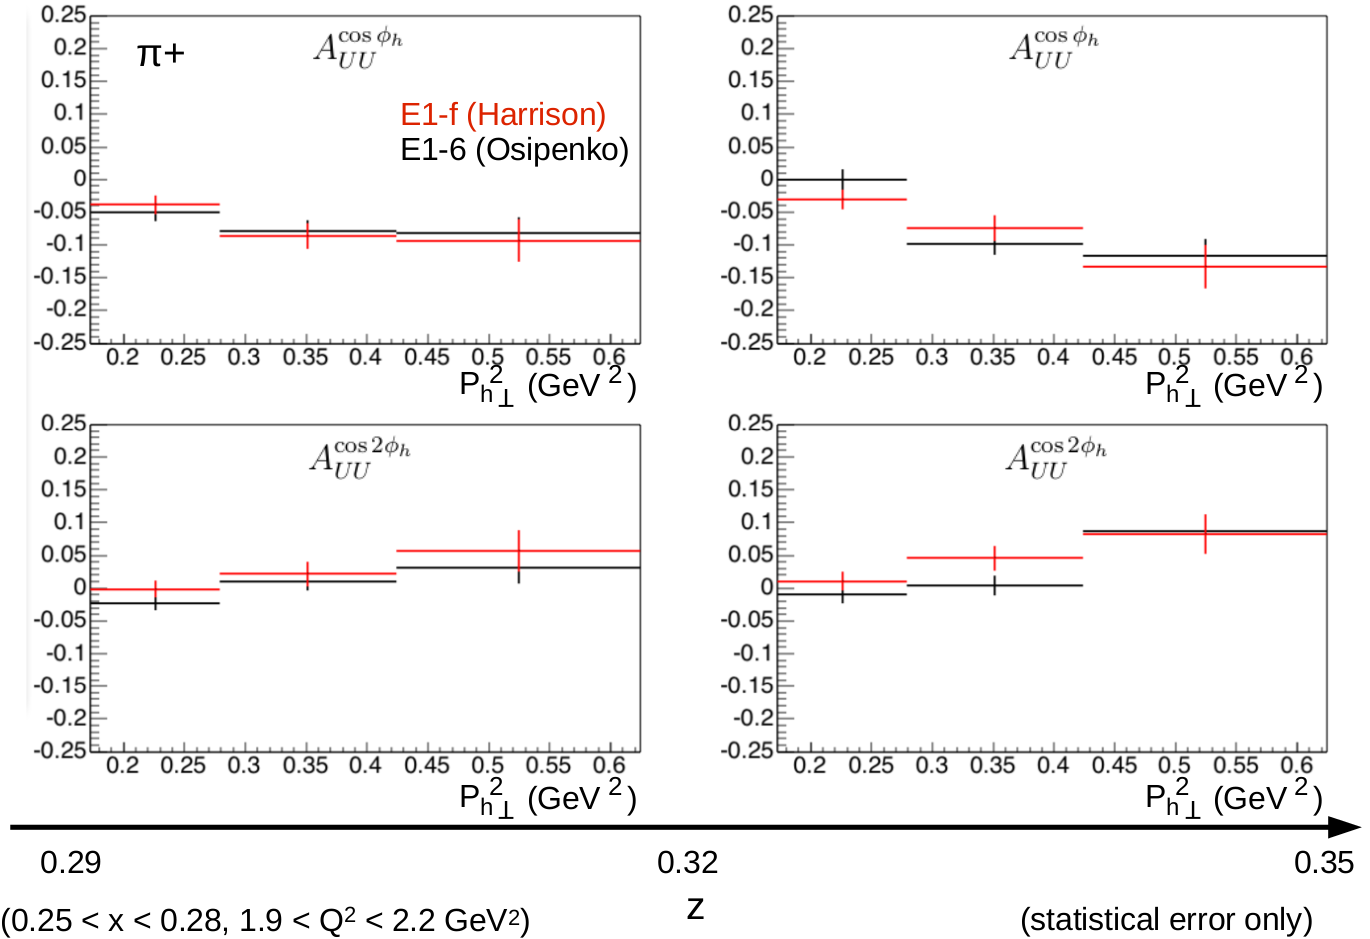
\includegraphics[width=8.5in]{figures/osipenkoComparisonVPT2_2zBins.png}
\caption{$A_{UU}^{\cos \phi_h}$ (top row) and $A_{UU}^{\cos 2\phi_h}$ (bottom row) vs $P_{h\perp}^2$ for two $z$ bins ($0.29 < z < 0.32$ (left column) and $0.32 < z < 0.35$ (right column)) for the $\pi^+$ channel for E1-f (red points) and E1-6 (black points). Only the statistical error bars are shown here.}
\label{fig:osipenkoComparisonVPT2_2zBins}
\end{sidewaysfigure}
%
\clearpage

